% Note that the a4paper option is mainly intended so that authors in
% countries using A4 can easily print to A4 and see how their papers will
% look in print - the typesetting of the document will not typically be
% affected with changes in paper size (but the bottom and side margins will).
% Use the testflow package mentioned above to verify correct handling of
% both paper sizes by the user's LaTeX system.
%
% Also note that the "draftcls" or "draftclsnofoot", not "draft", option
% should be used if it is desired that the figures are to be displayed in
% draft mode.
%
\documentclass[conference]{IEEEtran}
% Add the compsoc option for Computer Society conferences.
%
% If IEEEtran.cls has not been installed into the LaTeX system files,
% manually specify the path to it like:
% \documentclass[conference]{../sty/IEEEtran}





% Some very useful LaTeX packages include:
% (uncomment the ones you want to load)


% *** MISC UTILITY PACKAGES ***
%
%\usepackage{ifpdf}
% Heiko Oberdiek's ifpdf.sty is very useful if you need conditional
% compilation based on whether the output is pdf or dvi.
% usage:
% \ifpdf
%   % pdf code
% \else
%   % dvi code
% \fi
% The latest version of ifpdf.sty can be obtained from:
% http://www.ctan.org/tex-archive/macros/latex/contrib/oberdiek/
% Also, note that IEEEtran.cls V1.7 and later provides a builtin
% \ifCLASSINFOpdf conditional that works the same way.
% When switching from latex to pdflatex and vice-versa, the compiler may
% have to be run twice to clear warning/error messages.






% *** CITATION PACKAGES ***
%
\usepackage{cite}
% cite.sty was written by Donald Arseneau
% V1.6 and later of IEEEtran pre-defines the format of the cite.sty package
% \cite{} output to follow that of IEEE. Loading the cite package will
% result in citation numbers being automatically sorted and properly
% "compressed/ranged". e.g., [1], [9], [2], [7], [5], [6] without using
% cite.sty will become [1], [2], [5]--[7], [9] using cite.sty. cite.sty's
% \cite will automatically add leading space, if needed. Use cite.sty's
% noadjust option (cite.sty V3.8 and later) if you want to turn this off
% such as if a citation ever needs to be enclosed in parenthesis.
% cite.sty is already installed on most LaTeX systems. Be sure and use
% version 4.0 (2003-05-27) and later if using hyperref.sty. cite.sty does
% not currently provide for hyperlinked citations.
% The latest version can be obtained at:
% http://www.ctan.org/tex-archive/macros/latex/contrib/cite/
% The documentation is contained in the cite.sty file itself.






% *** GRAPHICS RELATED PACKAGES ***
%
\ifCLASSINFOpdf
  \usepackage[pdftex]{graphicx}
  % declare the path(s) where your graphic files are
  % \graphicspath{{../pdf/}{../jpeg/}}
  % and their extensions so you won't have to specify these with
  % every instance of \includegraphics
  % \DeclareGraphicsExtensions{.pdf,.jpeg,.png}
\else
  % or other class option (dvipsone, dvipdf, if not using dvips). graphicx
  % will default to the driver specified in the system graphics.cfg if no
  % driver is specified.
  % \usepackage[dvips]{graphicx}
  % declare the path(s) where your graphic files are
  % \graphicspath{{../eps/}}
  % and their extensions so you won't have to specify these with
  % every instance of \includegraphics
  % \DeclareGraphicsExtensions{.eps}
\fi
% graphicx was written by David Carlisle and Sebastian Rahtz. It is
% required if you want graphics, photos, etc. graphicx.sty is already
% installed on most LaTeX systems. The latest version and documentation
% can be obtained at: 
% http://www.ctan.org/tex-archive/macros/latex/required/graphics/
% Another good source of documentation is "Using Imported Graphics in
% LaTeX2e" by Keith Reckdahl which can be found at:
% http://www.ctan.org/tex-archive/info/epslatex/
%
% latex, and pdflatex in dvi mode, support graphics in encapsulated
% postscript (.eps) format. pdflatex in pdf mode supports graphics
% in .pdf, .jpeg, .png and .mps (metapost) formats. Users should ensure
% that all non-photo figures use a vector format (.eps, .pdf, .mps) and
% not a bitmapped formats (.jpeg, .png). IEEE frowns on bitmapped formats
% which can result in "jaggedy"/blurry rendering of lines and letters as
% well as large increases in file sizes.
%
% You can find documentation about the pdfTeX application at:
% http://www.tug.org/applications/pdftex





% *** MATH PACKAGES ***
%
\usepackage[cmex10]{amsmath}
% A popular package from the American Mathematical Society that provides
% many useful and powerful commands for dealing with mathematics. If using
% it, be sure to load this package with the cmex10 option to ensure that
% only type 1 fonts will utilized at all point sizes. Without this option,
% it is possible that some math symbols, particularly those within
% footnotes, will be rendered in bitmap form which will result in a
% document that can not be IEEE Xplore compliant!
%
% Also, note that the amsmath package sets \interdisplaylinepenalty to 10000
% thus preventing page breaks from occurring within multiline equations. Use:
%\interdisplaylinepenalty=2500
% after loading amsmath to restore such page breaks as IEEEtran.cls normally
% does. amsmath.sty is already installed on most LaTeX systems. The latest
% version and documentation can be obtained at:
% http://www.ctan.org/tex-archive/macros/latex/required/amslatex/math/





% *** SPECIALIZED LIST PACKAGES ***
%
%\usepackage{algorithmic}
% algorithmic.sty was written by Peter Williams and Rogerio Brito.
% This package provides an algorithmic environment fo describing algorithms.
% You can use the algorithmic environment in-text or within a figure
% environment to provide for a floating algorithm. Do NOT use the algorithm
% floating environment provided by algorithm.sty (by the same authors) or
% algorithm2e.sty (by Christophe Fiorio) as IEEE does not use dedicated
% algorithm float types and packages that provide these will not provide
% correct IEEE style captions. The latest version and documentation of
% algorithmic.sty can be obtained at:
% http://www.ctan.org/tex-archive/macros/latex/contrib/algorithms/
% There is also a support site at:
% http://algorithms.berlios.de/index.html
% Also of interest may be the (relatively newer and more customizable)
% algorithmicx.sty package by Szasz Janos:
% http://www.ctan.org/tex-archive/macros/latex/contrib/algorithmicx/




% *** ALIGNMENT PACKAGES ***
%
%\usepackage{array}
% Frank Mittelbach's and David Carlisle's array.sty patches and improves
% the standard LaTeX2e array and tabular environments to provide better
% appearance and additional user controls. As the default LaTeX2e table
% generation code is lacking to the point of almost being broken with
% respect to the quality of the end results, all users are strongly
% advised to use an enhanced (at the very least that provided by array.sty)
% set of table tools. array.sty is already installed on most systems. The
% latest version and documentation can be obtained at:
% http://www.ctan.org/tex-archive/macros/latex/required/tools/


% IEEEtran contains the IEEEeqnarray family of commands that can be used to
% generate multiline equations as well as matrices, tables, etc., of high
% quality.




% *** SUBFIGURE PACKAGES ***
\ifCLASSOPTIONcompsoc
  \usepackage[caption=false,font=normalsize,labelfont=sf,textfont=sf]{subfig}
\else
  \usepackage[caption=false,font=footnotesize]{subfig}
\fi
% subfig.sty, written by Steven Douglas Cochran, is the modern replacement
% for subfigure.sty, the latter of which is no longer maintained and is
% incompatible with some LaTeX packages including fixltx2e. However,
% subfig.sty requires and automatically loads Axel Sommerfeldt's caption.sty
% which will override IEEEtran.cls' handling of captions and this will result
% in non-IEEE style figure/table captions. To prevent this problem, be sure
% and invoke subfig.sty's "caption=false" package option (available since
% subfig.sty version 1.3, 2005/06/28) as this is will preserve IEEEtran.cls
% handling of captions.
% Note that the Computer Society format requires a larger sans serif font
% than the serif footnote size font used in traditional IEEE formatting
% and thus the need to invoke different subfig.sty package options depending
% on whether compsoc mode has been enabled.
%
% The latest version and documentation of subfig.sty can be obtained at:
% http://www.ctan.org/tex-archive/macros/latex/contrib/subfig/




% *** FLOAT PACKAGES ***
%
\usepackage{fixltx2e}
% fixltx2e, the successor to the earlier fix2col.sty, was written by
% Frank Mittelbach and David Carlisle. This package corrects a few problems
% in the LaTeX2e kernel, the most notable of which is that in current
% LaTeX2e releases, the ordering of single and double column floats is not
% guaranteed to be preserved. Thus, an unpatched LaTeX2e can allow a
% single column figure to be placed prior to an earlier double column
% figure. The latest version and documentation can be found at:
% http://www.ctan.org/tex-archive/macros/latex/base/

\usepackage{float}
\usepackage{stfloats}
% stfloats.sty was written by Sigitas Tolusis. This package gives LaTeX2e
% the ability to do double column floats at the bottom of the page as well
% as the top. (e.g., "\begin{figure*}[!b]" is not normally possible in
% LaTeX2e). It also provides a command:
%\fnbelowfloat
% to enable the placement of footnotes below bottom floats (the standard
% LaTeX2e kernel puts them above bottom floats). This is an invasive package
% which rewrites many portions of the LaTeX2e float routines. It may not work
% with other packages that modify the LaTeX2e float routines. The latest
% version and documentation can be obtained at:
% http://www.ctan.org/tex-archive/macros/latex/contrib/sttools/
% Do not use the stfloats baselinefloat ability as IEEE does not allow
% \baselineskip to stretch. Authors submitting work to the IEEE should note
% that IEEE rarely uses double column equations and that authors should try
% to avoid such use. Do not be tempted to use the cuted.sty or midfloat.sty
% packages (also by Sigitas Tolusis) as IEEE does not format its papers in
% such ways.
% Do not attempt to use stfloats with fixltx2e as they are incompatible.
% Instead, use Morten Hogholm'a dblfloatfix which combines the features
% of both fixltx2e and stfloats:
%
% \usepackage{dblfloatfix}
% The latest version can be found at:
% http://www.ctan.org/tex-archive/macros/latex/contrib/dblfloatfix/




% *** PDF, URL AND HYPERLINK PACKAGES ***
%
\usepackage{url}
%\usepackage{authblk}
\usepackage{textcomp}

% correct bad hyphenation here
\hyphenation{op-tical net-works semi-conduc-tor}


\begin{document}
%
% paper title
% can use linebreaks \\ within to get better formatting as desired
% Do not put math or special symbols in the title.
\title{Software Architecture Development and Implementation of a Synchrophasor-based Real-Time Oscillation Damping Control System}

%
%Old title Software Architecture Development and Implementation of a Synchrophasor-based Real-Time Oscillation Damping Control System
% author names and affiliations
% use a multiple column layout for up to three different
% affiliations
\author{\IEEEauthorblockN{Eldrich Rebello}
\IEEEauthorblockA{KTH Royal Institute of Technology\\
Stockholm, Sweden\\
Email: rebello@kth.se}
\thanks{And so on}
\and
\IEEEauthorblockN{Luigi Vanfretti}
\IEEEauthorblockA{KTH Royal Institute of Technology\\
\& Statnett SF\\
Email: luigi.vanfretti@statnett.no}
\and
\IEEEauthorblockN{Md. Shoaib Almas}
\IEEEauthorblockA{KTH Royal Institute of Technology\\
Stockholm, Sweden\\
Email: msalmas@kth.se}
}
% conference papers do not typically use \thanks and this command
% is locked out in conference mode. If really needed, such as for
% the acknowledgment of grants, issue a \IEEEoverridecommandlockouts
% after \documentclass

% use for special paper notices
%\IEEEspecialpapernotice{(Invited Paper)}

% make the title area
\maketitle

% As a general rule, do not put math, special symbols or citations
% in the abstract
\begin{abstract}

%The Phasor Power Oscillation Damping (Phasor POD) algorithm has been demonstrated to be effective at damping inter-area power system oscillations. Present implementations of the algorithm have been either in offline or real-time \textsc{Simulink} simulations. Previous research has demonstrated that wide-area signals are effective at achieving enhanced damping of inter-area modes. This work documents the design proposal and revision process for a real-time hardware prototype of the Phasor-POD algorithm on a Compact Reconfigurable Input Output (cRIO) controller from National Instruments. The real-world applicability of this design and the challenges faced together with the solutions implemented are also investigated.\\

Low-frequency, electro-mechanically induced, inter-area oscillations have in the past, posed a serious threat to the stability of interconnected power systems. Wide Area Monitoring, Protection and Control (WAMPAC) systems based on wide-area measurements such as synchrophasor (C37.118) data can be exploited to address the inter-area oscillation problem. This work develops a modular software architecture for a prototype WAMPAC control system. A Compact Reconfigurable Input Output (cRIO) controller from National Instruments is used to implement the real-time prototype. This paper presents the design process followed for the development of the software architecture. The design method followed a three step process of design proposal, refinement and attempted implementation. Results from each iteration are used to improve the next. The goals of the design, the challenges faced and the refinements necessary are presented. The details of the final implementation in LabVIEW are also documented.

%The modern power grid is increasingly being used under operating conditions of increasing stress for which it was not designed. The increasing penetration levels of variable energy sources such as wind present significant grid stability issues. One of these stability issues is the phenomenon of low frequency, electro-mechanically induced, inter-area oscillations. Simulations have demonstrated the potential of Wide Area Measurement Signals (WAMS)-based Power Oscillation Damping (POD) in achieving improved electromechanical mode damping compared to traditional, local signal based, Power System Stabilizers (PSS). This paper documents the software architecture that was envisaged, refined and finally implemented in the development of a real-time implementation of the Phasor-Power Oscillation Damper (Phasor POD).Tests were conducted to verify the working and performance of the real-time algorithm implementation. The challenges faced and the solutions implemented are also documented here.
\end{abstract}

% no keywords




% For peer review papers, you can put extra information on the cover
% page as needed:
% \ifCLASSOPTIONpeerreviewPS
% \begin{center} \bfseries EDICS Category: 3-BBND \end{center}
% \fi
%
% For peerreview papers, this IEEEtran command inserts a page break and
% creates the second title. It will be ignored for other modes.
\IEEEpeerreviewmaketitle

\section{Introduction}
%\subsection{Motivation}
The growth of power system interconnections between previously isolated areas has given rise to the phenomenon of inter-area oscillations. These are low frequency (0.1-2 Hz.) oscillations where the generators of one synchronous area oscillate against those of another area. Damping for these oscillations is generally poor and, if allowed to grow, can lead to disconnection of the ties or a collapse of the power system. A famous example of the latter was the August 1996 blackout of the WSCC system in the USA \cite{NAERC}. Although the purpose of system interconnection was to increase stability, the present situation of the power system incorporates renewable energy sources and power trading corridors, both of which impact system stability.

\begin{figure*}[htb]
\centering
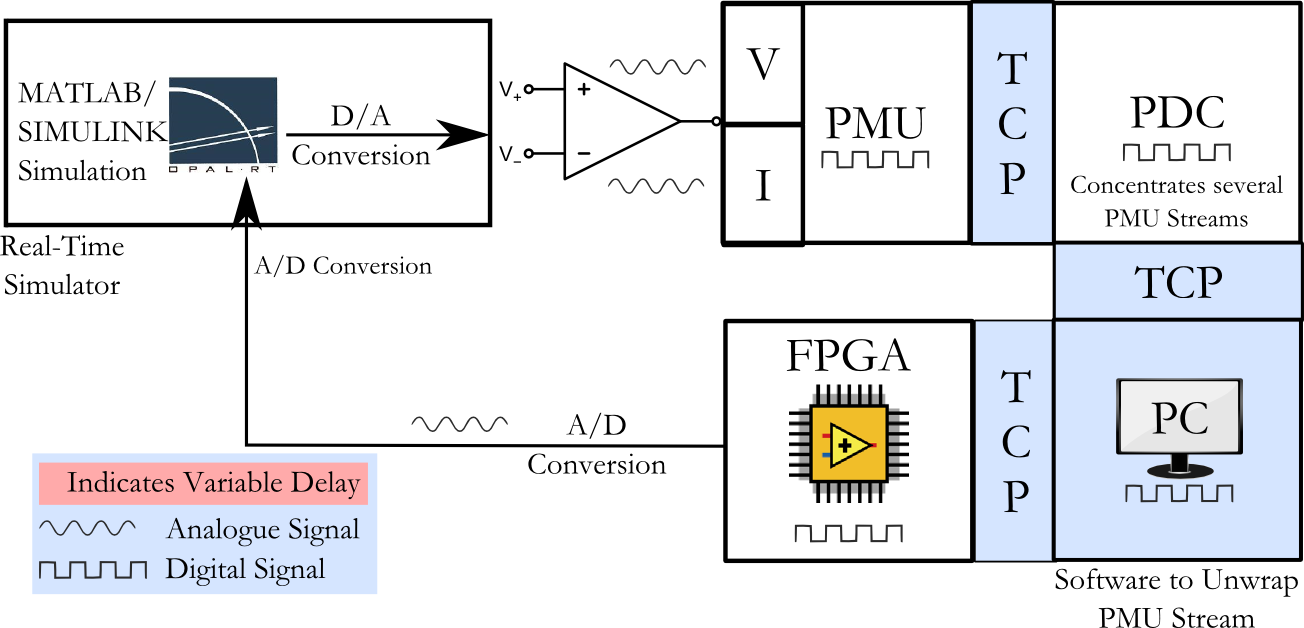
\includegraphics[width=4in]{DataFlow.png}
\caption{Data flow path with digital and analogue components indicated}
\label{Data_path}
\end{figure*}

\subsection{Previous Experiences}
Locally available signals such as active power can be used in devices such as Power System Stabilisers (PSS). While effective at damping intra-area modes with good observability these may not be as effective at damping inter-area modes \cite{WAPODNorway} \cite{localREMcomparison}. A theoretical analysis of the advantages of using wide-area signals as a damping input is presented in \cite{Yuwa}. Field-test experiences with WAPOD controllers from Norway and China are presented in \cite{WAPODNorway} and \cite{WAPODChina} respectively. Although these initial field tests show promising results, the wide-area control systems tested so far have been implemented by extending the installed control system of an existing device (e.g. an SVC, see \cite{WAPODNorway}) to receive synchrophasor data, process it and to then feed the control algorithm. To the knowledge of the authors, there has not been any reported attempt at designing a general purpose, wide-area control system, starting from specifications and considering different hardware and software constraints. Such an approach is attractive as it can easily be adapted to different controllable elements thereby reducing implementation costs and facilitating straightforward development.
%\vspace{-0.7em}
\subsection{Contributions}
The goal of this paper is to document the software architecture development process and challenges faced in the real-time implementation of a wide-area control system. \"{A}ngquist and Gama's\cite{PhasorPOD} Phasor Power Oscillation (Phasor POD) algorithm was chosen based on the operational requirements and control system design constraints. The developed prototype is termed a Wide Area Power Oscillation Damper \footnote{Historically, damping stabilizers have been termed WAPOD where the P represents a measurement of active power through the line. In such context, active power is used as a controller input signal. Although this term is not accurate when other quantities are used as control inputs or feedback signals, the term is used here to maintain consistency with existing literature.} (WAPOD). For purposes of comparison, the real-time \textsc{Simulink} implementation of the Phasor POD algorithm by Almas and Vanfretti \cite{PhasorPODImplement} is used as a benchmark. The software architecture designed is implemented in LabVIEW on a real-time controller from National Instruments. To test the developed controller, the two-area four-machine model developed by Klein, Rogers and Kundur \cite{KundurTwoArea} is used as a test-case and is modified to fit the requirements of experimental testing. A Hardware-in-the-loop experiment is constructed around the e\textsc{MEGASIM} real-time simulator from OPAL-RT \cite{OPALemegasim} with the two-area model running in real-time, physical PMUs and a synchrophasor-based Phasor-POD algorithm running on a cRIO (Figure \ref{Data_path}).


\subsection{Paper Outline}
This paper is organised as follows. Section \ref{background} outlines the hardware and software components used together with an overview of the Phasor POD algorithm implemented. Section \ref{arch} examines the details of the architecture developed for this controller and the various stages of refinement and changes made to it. Section \ref{HILtest} details the different sections of LabVIEW code written and finally conclusions are drawn in Section \ref{conclusion}.

\section{Background}\label{background}

\subsection{Phasor POD Algorithm}
This algorithm\cite{PhasorPOD} was selected due to its wide applicability and the fact that it does not depend on the network model or updated knowledge of the network topology. Typical model-linearisation based damping algorithms rely on computer-intensive calculations and are often valid for a particular network operating point. In contrast, the Phasor-POD algorithm only requires knowledge of the inter-area oscillation frequency, which is generally known from system studies or can be determined from synchrophasor measurements \cite{TaskForce}. Consider Equation \ref{PODEqn}, which represents a general signal $s(t)$, as an average valued component and an oscillating component.
%The Phasor-POD algorithm was developed by \"{A}ngquist and Gama\cite{PhasorPOD} and forms the core of this work.
\begin{equation}
%\begin{multlined}
s(t)={s}_{avg}+\mathrm{Re}\left\{{\stackrel{\to }{s}}_{ph}\cdot {e}^{{jwt}}\right\}
%\mbox{where, } {\stackrel{\to }{s}}_{ph} \mbox{ is a complex phasor, rotating at the frequency }\\ \omega
\label{PODEqn}
%\end{multlined}
\end{equation}
%In the two-area network used here, the inter-area oscillation frequency is known to be 0.64Hz.
\noindent{where} $\stackrel{\to}{s}_{ph}$ is a complex phasor, rotating at the frequency $\omega$ \cite{PhasorPOD}. The Phasor-POD algorithm uses the known oscillation frequency to set up a co-orindate system rotating at this frequency and continuously extracts a phasor representing the oscillation\cite{PhasorPOD}. The implementation of the algorithm used here is based on Almas and Vanfretti's \textsc{Simulink} implementation \cite{PhasorPODImplement}. %and uses three inputs : the search frequency, $\omega_{cs1}$ and the sampling time $T_{s}$, the phase correction $alpha$ in addition to a signal scaling factor.

\subsection{Hardware}
\subsubsection{Real-Time Controller} The real-time implementation of the Phasor-POD algorithm in this work is based on the Compact Reconfigurable Input Output (cRIO) controller from National Instruments. The cRIO 9081 is used to implement the algorithm. It has an on-board Field Programmable Gate Array (FPGA) in addition to a 1.06 GHz. Intel Celeron processor for real-time control applications\cite{cRIO9081}.

\subsubsection{Phasor Measurement Units}
The inputs to the real-time controller were taken from an IEEEC37.118-compliant synchrophasor data stream. Measurement data for this stream was generated by two PMU's which monitor three-phase currents and voltages at different points on the power network. In this work, two cRIO9076 real-time controllers \cite{cRIO9081} were deployed as PMUs\cite{PMUMario}.

\subsubsection{Real-Time Simulator}
The e\textsc{megasim} real-time simulator from OPAL-RT \cite{OPALemegasim} was used for simulating the two-area network in real-time. Figure \ref{Data_path} presents the entire signal path including the external, closed-loop controller.

%\subsubsection*{Software}
%The test-case network model used here was a version of the Klein-Rogers-Kundur two-area system implemented in a \textsc{Simulink} demo available with SimPowerSystems\cite{SIMULINKOnline}. This was modified to include an average-valued SVC model, identical to that used in \cite{PhasorPODImplement}. The software on the cRIO was written using LabView's Real-Time modules. Software development was done on a workstation computer. Code was loaded on the various devices (cRIO contollers, RT Simulator) over a TCP network.


\section{Architecture Development Process}\label{arch}

Before beginning the development process, a software development methodology was adopted with the aim of streamlining the process\footnote{There are many software development methods that could be adopted. However, for this specific application (i.e a PMU-based WAPOD), none of them have been reported and used in available literature. The process here was favoured over the others due to the availability and limitations of the hardware-in-the-loop experimental testing facilities available at the SmarTS Lab\cite{SmarTSLab}}. The approach followed here is based on the Waterfall method detailed in \cite{WaterfallCoding}. The approach broadly includes the four steps from \cite{WaterfallCoding} 

\begin{figure}[htb]
\centering
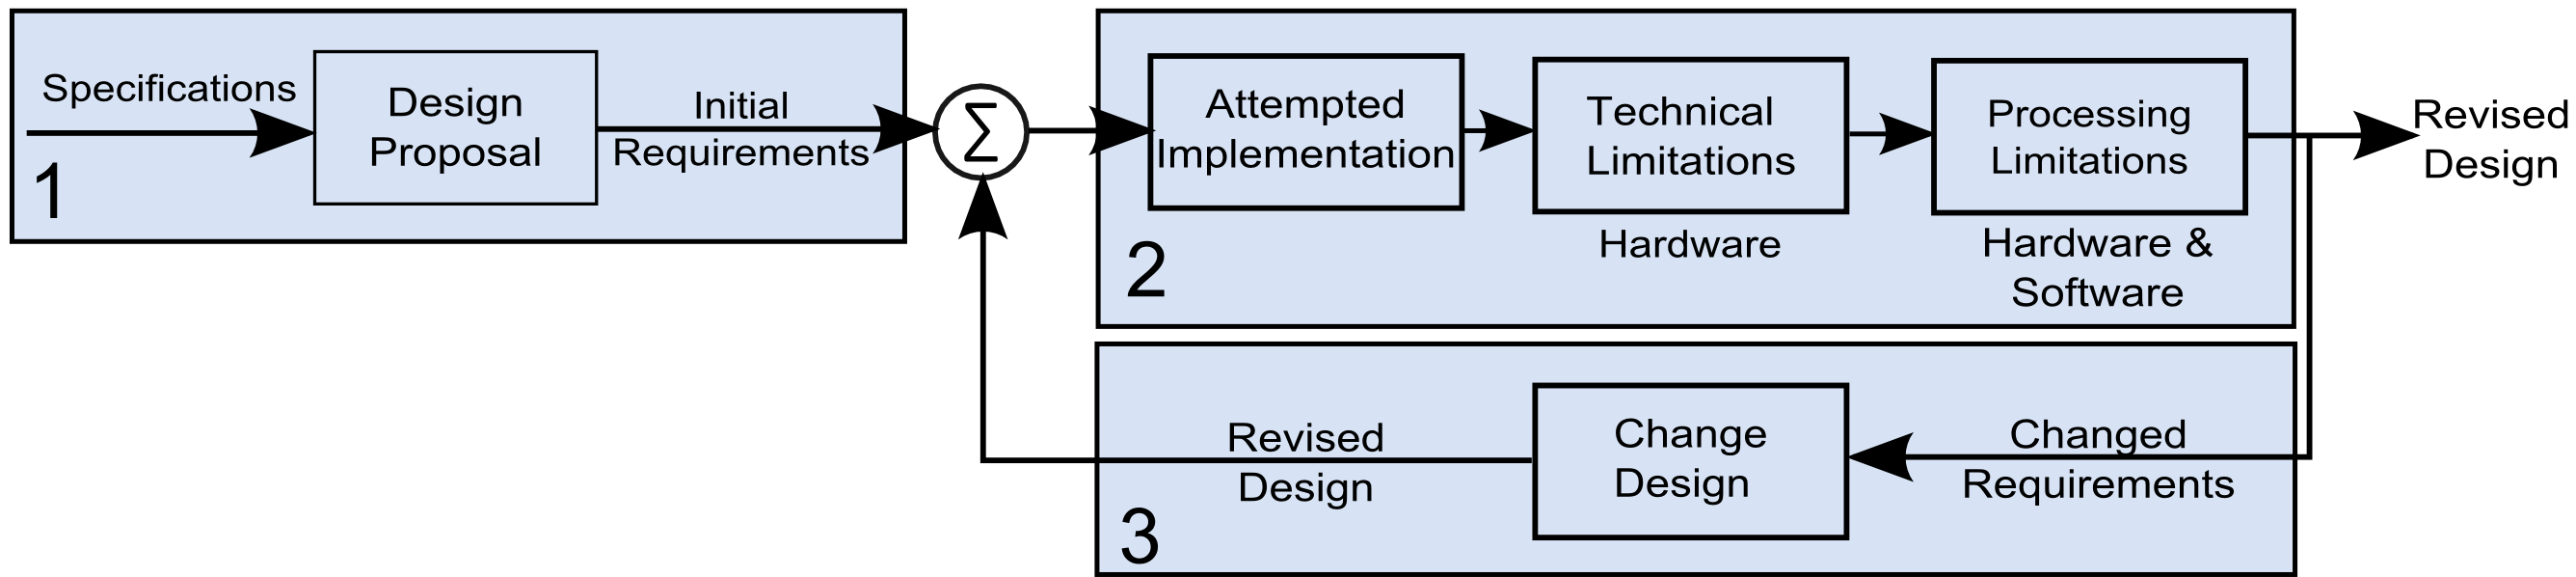
\includegraphics[width=3.45in]{RevisionFlow.png} 
\vspace{-0.5em}
\caption{General Iterative Revision Flow Diagram}
\label{fig:RevisionFlow}
\end{figure}

\begin{enumerate}
\item Initial Investigation
\item Requirements Definition
\item Architecture Design
\item Coding and Implementation
\item Experimental Testing to validate requirements
\end{enumerate}

An additional fifth step could be avoided thanks to the availability and use of HIL testing. The linear waterfall method was modified to be iterative so as to account for various constraints and to also account for revisions in the initial definition caused by these constraints. This iterative process is illustrated in Figure \ref{fig:RevisionFlow} and is realised for the specific application here, as illustrated in Figure \ref{fig:InitialArch}. Several reasons were behind the choice of an iterative design approach. Chief among them was the cRIO hardware itself. As an implementation on this hardware had not been attempted earlier, the limitations of the hardware were unknown. Based on the limitations faced during an implementation attempt, the design and features incorporated would be revised to fit within the limitations of the hardware. 
%\begin{figure}[!t]
%\centering
%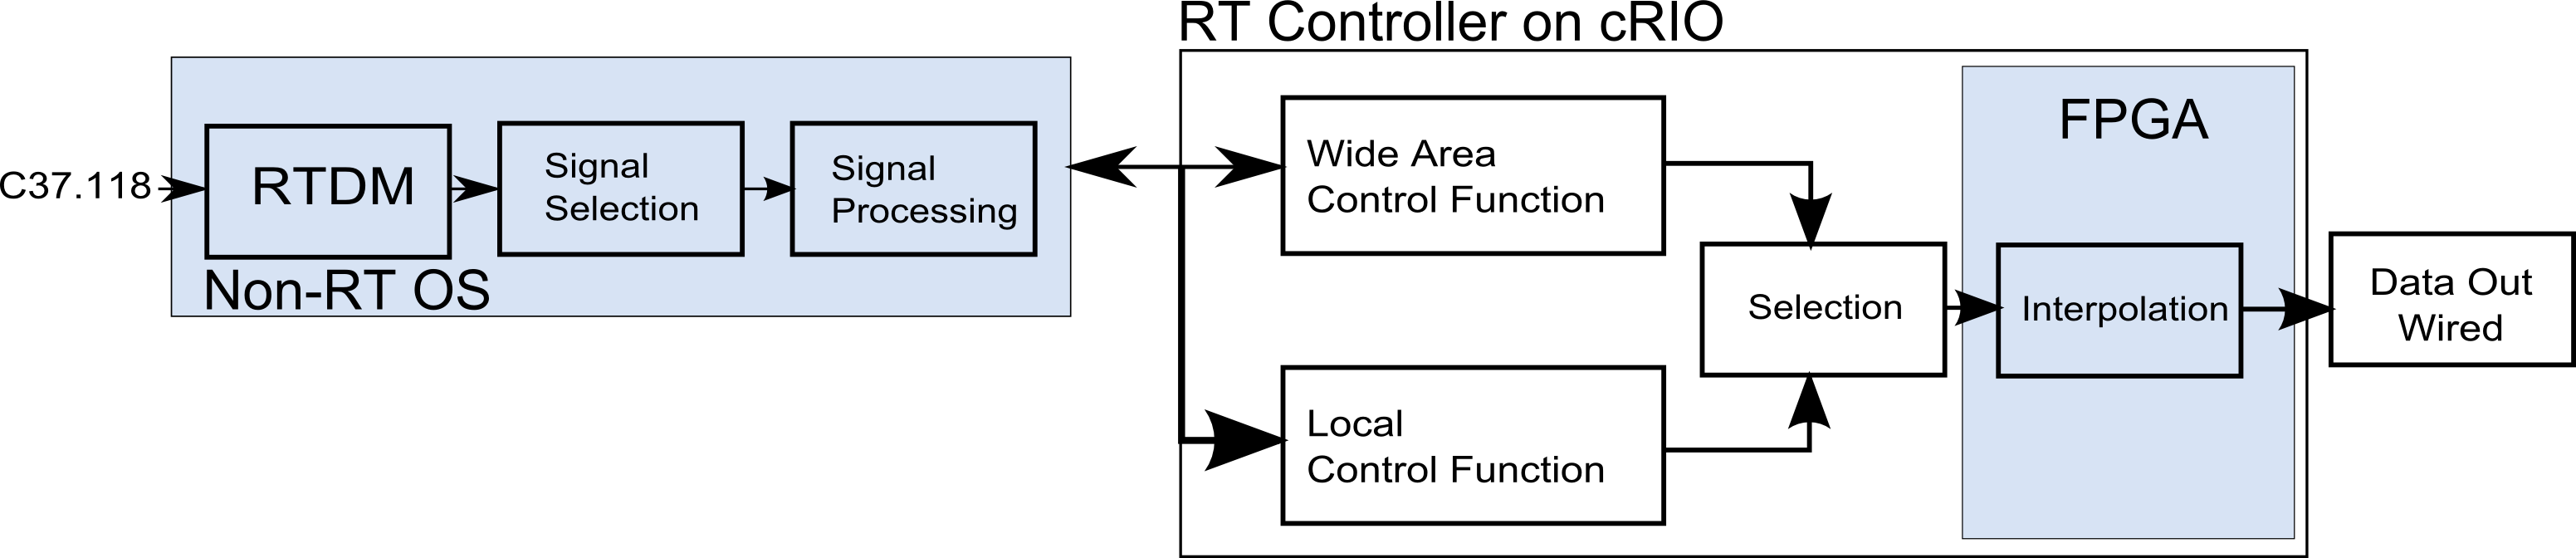
\includegraphics[width=3.5in]{Revision.png} 
%\caption{Iterative Revision Flow Diagram}
%\label{Revision1}
%\end{figure}
%\subsection{Controller Hardware Analysis}
%It was envisioned to use the cRIO platform from National Instruments. Add information about controller. Features of hardware controller that will affect design choices. Not PMU's as their problems are independent of platform actually used. This will focus on the problems of the cRIO used as a controller.
\subsection{Constraints}

Before defining requirements, the possible constraints at each stage of the test set-up were considered. The test set-up shown in Figure \ref{Data_path} is used to illustrate the constraints faced.

\subsubsection*{Differing Loop Rates}
The power system simulation running on the real-time simulator was executed at a loop rate of 50$\mu$s. This meant that the simulator generated new values for currents and voltages every 50$\mu$s. and would also expect data from the HIL system every 50$\mu$s. The constraint here was the data reporting rate of the PMU's used which was a maximum of 50 samples per second or one sample every 20ms. This was much slower that the 50$\mu$s. loop rate of the real-time simulator. 
\subsubsection*{FPGA Accuracy}
While the exact role of the FPGA in this implementation was not known in advance, it brought with it some limitations. Chief among these was the limitation on data accuracy due to the fact that all calculations together with circuit logic would be implemented in hardware.
%\vspace{-1em}
\section{Architecture Implementation and Refinement}
Figure \ref{fig:RevisionFlow} shows the three-stage design process with design proposal, implementation and revision. To begin with, only the controller specifications were available. These were used to draft a design proposal. An implementation attempt was made using this draft proposal. When the additional limits imposed by the software and hardware platforms were included, some goals of the original implementation needed to be revised. With these limitations, the original design was modified to generate a revised design. An attempt was then made to implement this revised design. As further limitations were encountered, the design was further modified. This iterative process was repeated till a working implementation was reached.

\subsubsection{Initial Design}
Initially, an autonomous, independent controller was envisaged. Such a controller would be able to receive IEEE C37.118 synchrophasor data directly over the communication network and extract measurement data. The architecture block diagram is shown in Figure  \ref{fig:InitialArch}. This controller was completely autonomous, with automated signal selection and processing. This design also incorporated two control functions, a wide area control function and a local control function. The wide area control function selected for implementation was the phasor-based oscillation damping control algorithm\cite{PhasorPOD}. The local control function would use locally available data in a manner similar to a Power System Stabiliser (PSS). Automatic switching between the two functions and automated input signal selection was also considered. If the signal to noise ratio in the wide area signal deteriorated or if the signal delay became prohibitively high, the controller would automatically switch to the local signal or another wide-area signal. The principal consideration in this design was the limited resources available on the FPGA and the complexity of the algorithms to be implemented. This required implementation of all algorithms and computation sections on the RT section of the cRIO with the FPGA being used for interpolation only. %In addition, the RT controller chosen has tremendous flexibility as algorithms are implemented using software, rather than hardware as on the FPGA. The RT controller also has more storage space available to implement algorithms. %This design would be able to compute observability indices for the different input signals and then automatically select the one with the highest observability of a particular mode

%\begin{figure}[!b]
%\centering
%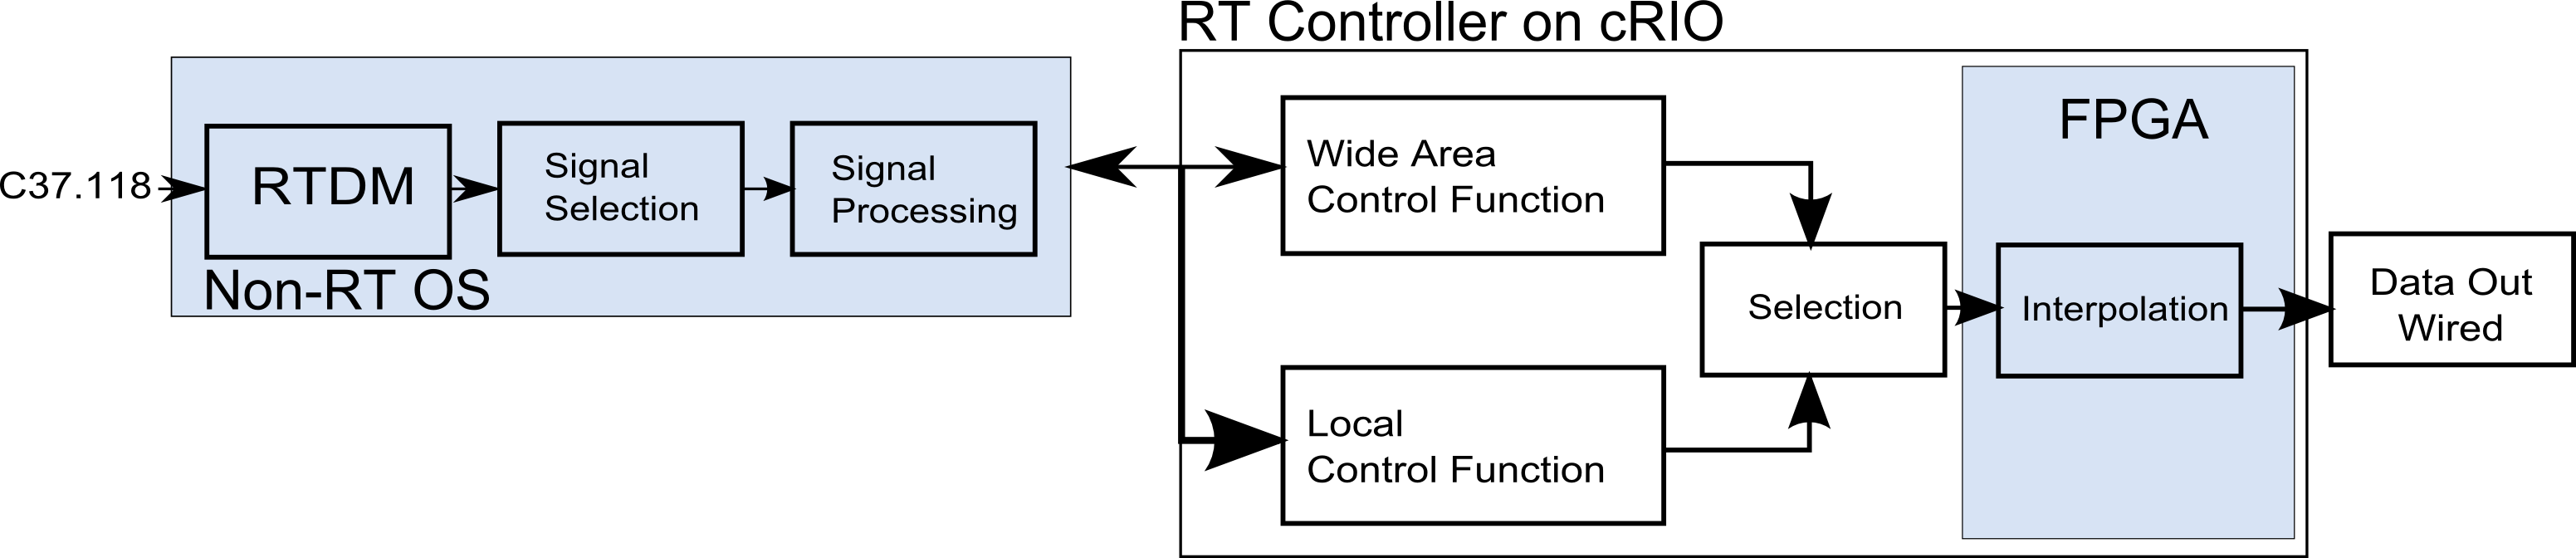
\includegraphics[width=3.5in]{Revision.png} 
%\caption{Iterative Revision Flow Diagram}
%\label{Revision1}
%\end{figure}

\subsubsection*{Challenges} This design was faced with a problem of differing loop rates. The real-time simulator runs at a 50$\mu$s time step. The fastest that the RT controller could run was 1ms. Data would thus be generated faster than the RT controller was able to process. The second problem was producing control output at the rate expected by the real-time simulator. The speed constraint of the RT controller meant that it would not be possible to use it to generate a control signal. To address this issue, this architecture envisaged using the FPGA to perform interpolation between successive data points. The FPGA would run at a loop rate of 50$\mu s$, to match the real-time simulator. The region between successive data points would be interpolated using a suitable interpolation algorithm. Data generated by the FPGA would be sent over the communication network back to the real-time simulator for use in the simulation. This design needed to be changed due to limitations of different components. 
%The RT controller on the cRIO is not capable of matching this speed.
\begin{figure}[htb]
\centering
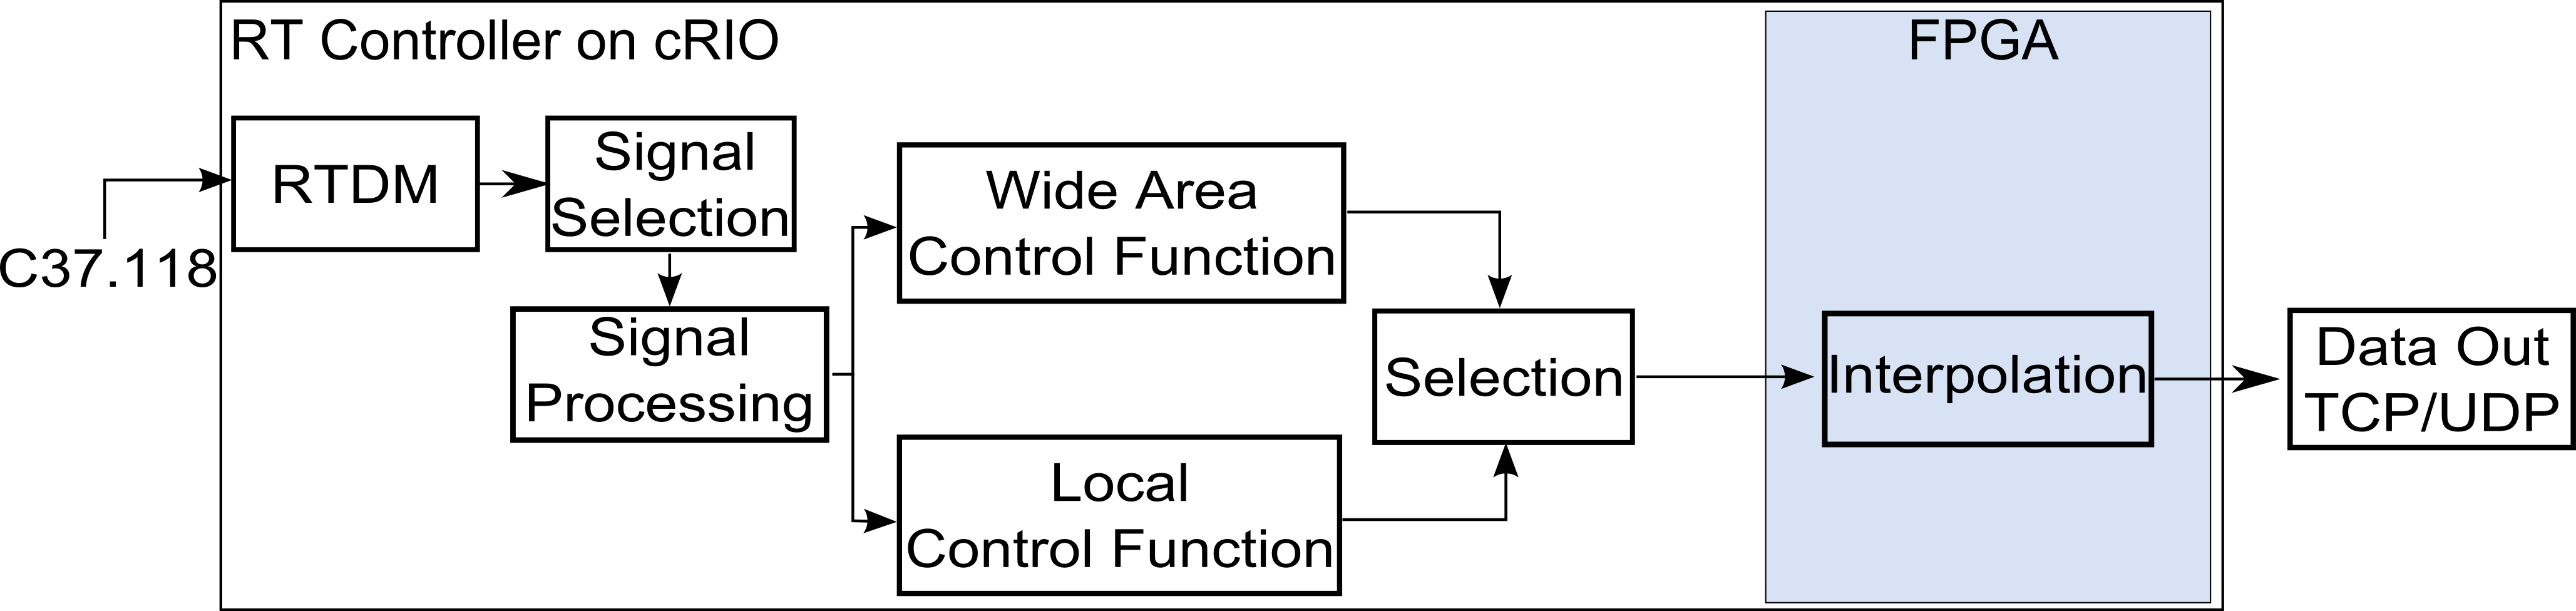
\includegraphics[width=3.5in]{InitialArch}
\vspace{-0.5em}
\caption{Initial Software Architecture}
\label{fig:InitialArch}
\end{figure}

One, no software was available to receive a synchrophasor stream and extract measurement data directly on the RT controller. This process had to be performed on a desktop computer running a real-time data mediator (Statnett's Synchrophasor Software Development Toolkit, $S^{3}DK$ \cite{SDK}) and LabVIEW. Once measurement data from the synchrophasor stream was available, it could be streamed to the real-time controller over the TCP/IP network using LabView's Shared Network Variables. Two, data generated by the FPGA could not be sent to the real-time simulator directly over the communication network. Though theoretically possible, further work is required. Also, for each successive data point received by the real-time controller, the FPGA would generate 400, interpolated, data points. Synchronising the process of generating the control signal and the use of the generated data on the real-time simulator is a complex task. Three, the process of data interpolation on the FPGA is computationally intensive. To achieve results better than with a simple linear interpolation, a history of past data points is required. This process is, in itself, complex and introduces further delay. It is, however, simpler than implementing the damping control algorithm on the FPGA. At this stage, FPGA limitations were the principal factor behind choosing to implement the Phasor-POD algorithm on the RT controller.

Four, an algorithm for automated signal selection based on observability indices had not been developed. In principle, this too, is possible and can be implemented on the real-time controller in the future when such an algorithm is developed and verified. The Phasor POD algorithm input parameters also change depending on the input used. An approach to determine these parameters iteratively or calculate them from input data is required. %This only adds to the complexity.

\subsubsection{Development and Revision}
\begin{figure}[htb]
\centering
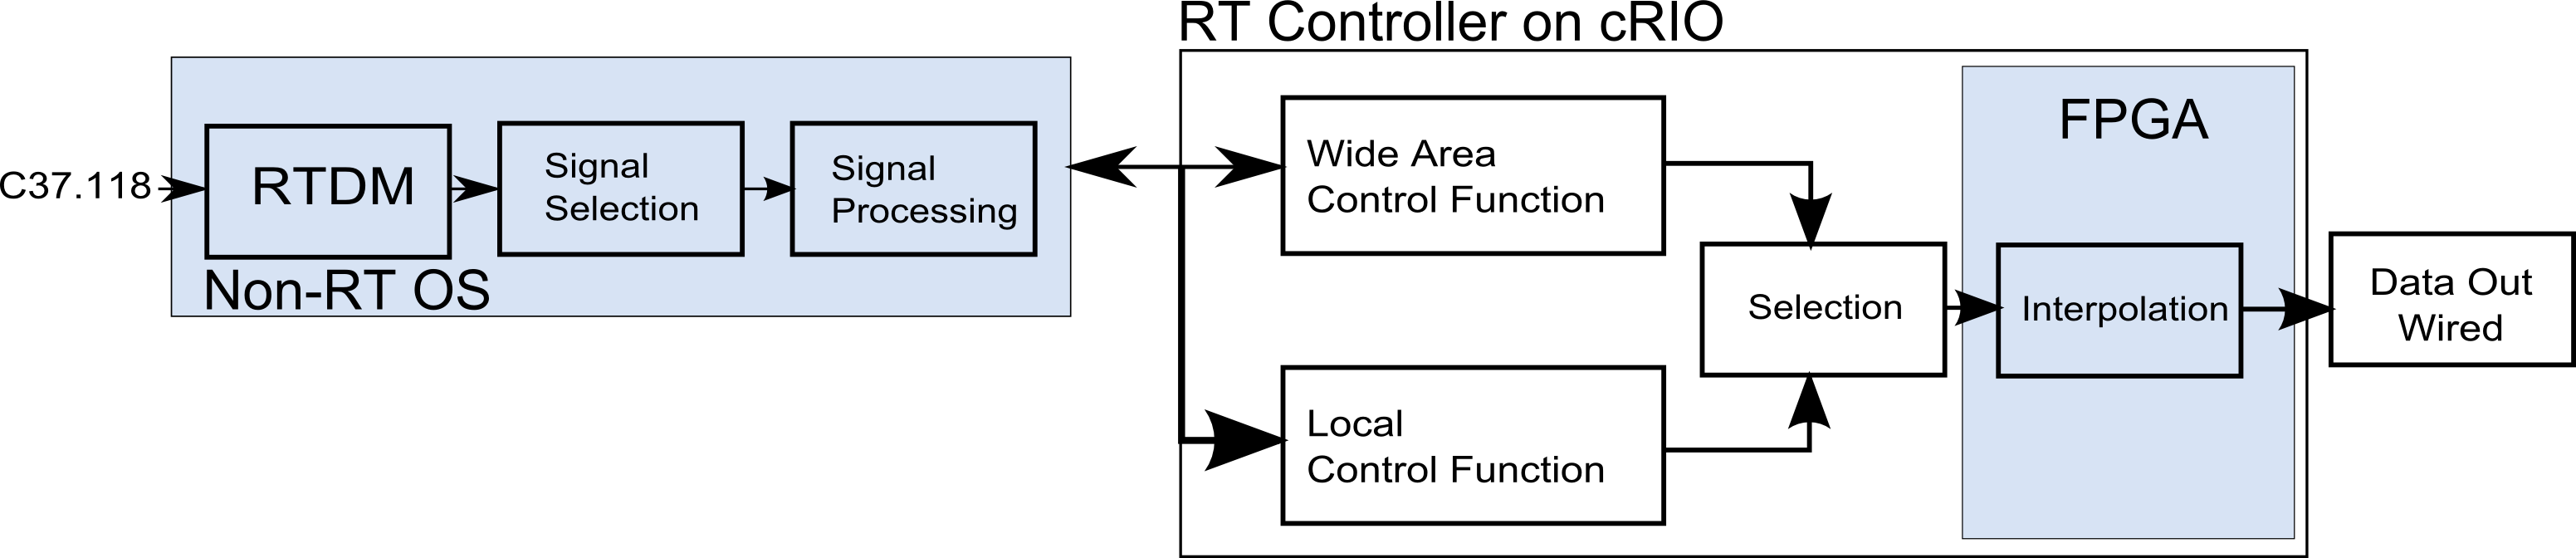
\includegraphics[width=3.5in]{Revision.png}
\vspace{-0.5em}
\caption{Revised Architecture}
\label{fig:Revision}
\end{figure}

With the limitations of the initial architecture in mind, the architecture was refined. The process of  extracting data from the synchrophasor stream was shifted to a workstation computer along with the processes of signal selection and processing. Once data was available, it was sent to the RT controller, over the  network. The damping control was kept on the RT controller with the FPGA performing the interpolation required to match the read-interval of the real-time simulator. Besides the damping control algorithm, a local control function was included on the RT controller. This revision is shown in Figure \ref{fig:Revision}. Here, the complexity of implementing an interpolation algorithm on the FPGA was examined in detail. An implementation was also attempted. It was determined that a simple linear interpolation algorithm would not be sufficiently accurate. An implementation of the damping control algorithm on the RT controller was also tested. The fastest loop rate that could be achieved was always in excess of 25ms. This was slower than the reporting rate of the PMUs. Communication between the cRIO and the RT simulator using TCP/IP was also abandoned. Analogue output signals of the FPGA were instead hard-wired to the real-time simulator's analogue inputs.
\subsubsection{Final Implementation}
%\begin{figure}[htb]
%\centering
%\includegraphics[width=1\linewidth]{./Final}
%\caption{Final Software Architecture as Implemented}
%\label{fig:Final}
%\end{figure}
%Further, the FPGA output was limited by the speed of the RT controller. 
\begin{figure}[htb]
\centering
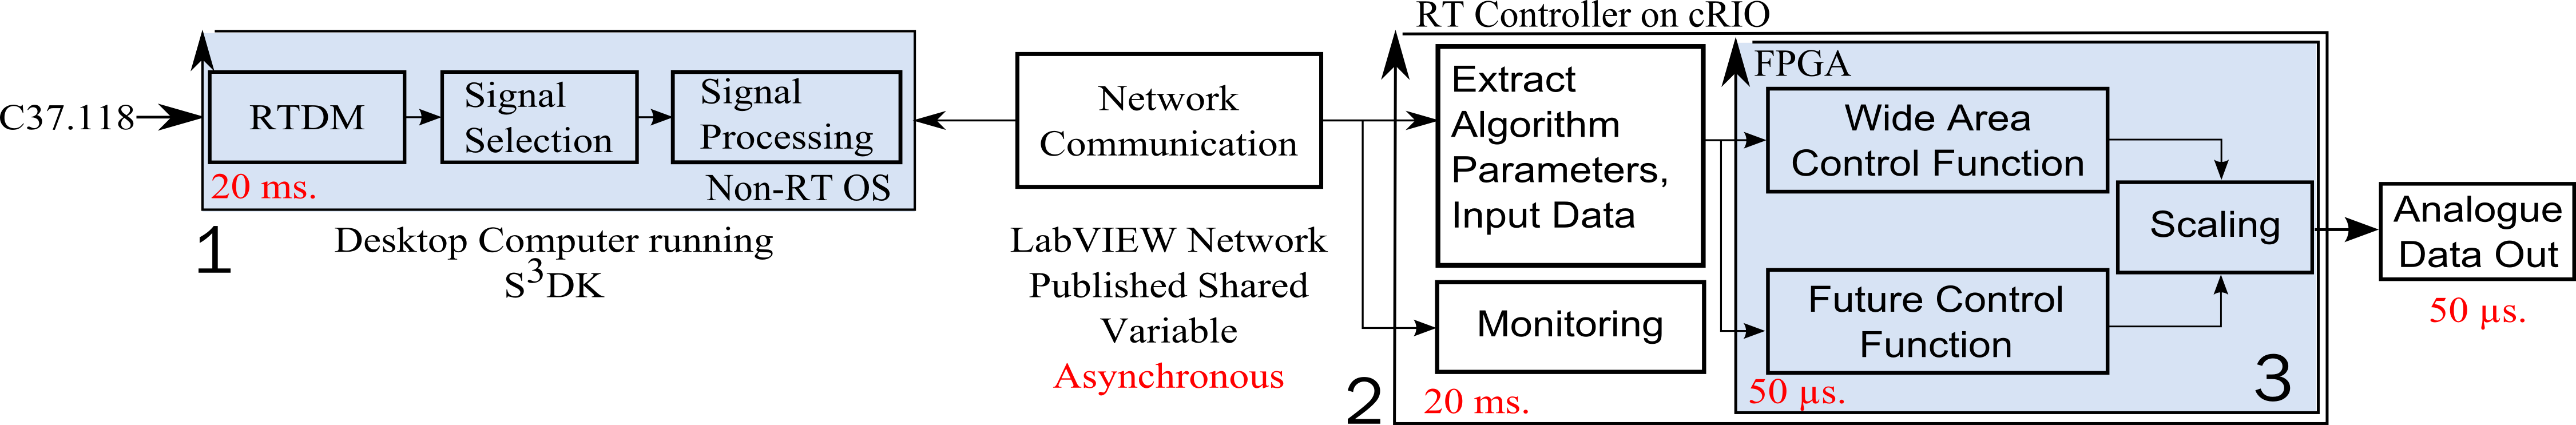
\includegraphics[width=3.5in]{Final_RT_Arch.png} 
\vspace{-0.5em}
\caption{Final Controller Architecture as Implemented}
\label{Final_arch}
\end{figure}

At this stage, the damping control algorithm was moved to the FPGA with the RT controller being used only for network communication and data monitoring. The  Phasor POD algorithm parameters and monitoring data would be sent over the network to the RT section of the controller. The local control function was also discarded as it was found to reduce the response speed of the RT controller. If needed and if space permits, the local control function can be implemented on the FPGA. The desired 50$\mu$s. data output rate could also be maintained as the FPGA was capable of response times of this order. The problem of differing data and loop rates was solved by implementing a basic sample-and-hold algorithm on the FPGA. Data would still be received from the RT controller every 20 ms. but the output would be held constant till the next data point was received and processed. With the Phasor POD algorithm implemented on the FPGA, resource utilization stood at 78\%. As with the previous design, the process of extracting data from the synchrophasor stream was done on a workstation computer. This (Figure \ref{Final_arch}) was the final architecture as implemented. %An outline of the FPGA code as implemented are shown in Figure \ref{FPGA_Blocks}.
%\begin{figure}[!htb]
%\centering
%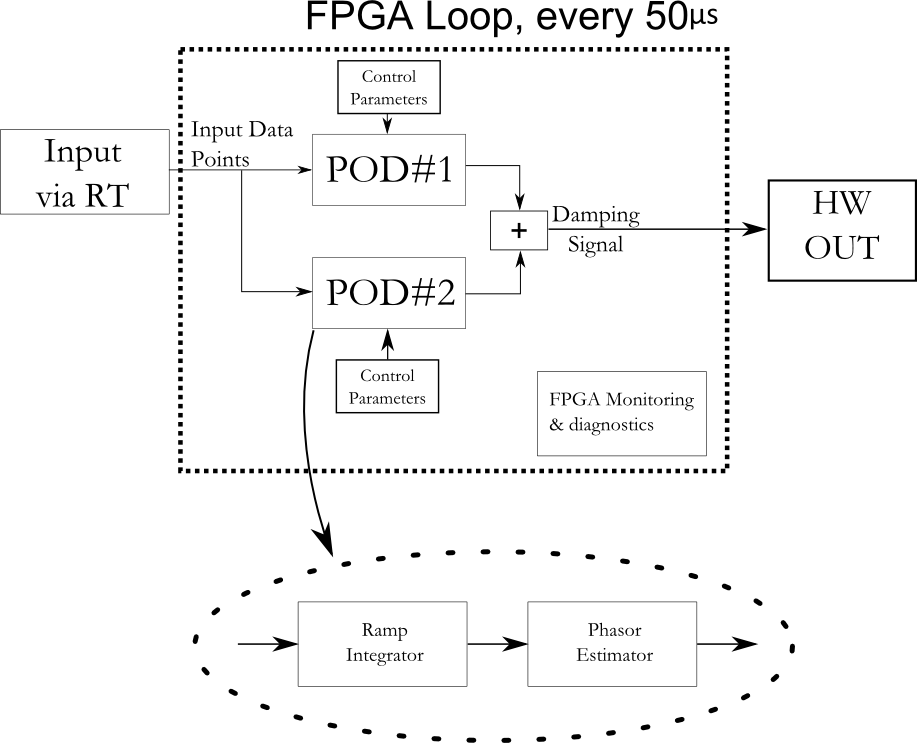
\includegraphics[width=3in]{FPGAOnly.png} 
%\caption{FPGA Software block diagram}
%\label{FPGA_Blocks}
%\end{figure}
\section{Architecture Implementation using the LabVIEW Platform} \label{HILtest}
The central part of implementing the architecture described here was the code written for the cRIO. This was written using the real-time and FPGA toolboxes available in LabVIEW\cite{cRIO9081}. Broadly speaking, three layers of code were written corresponding to labels 1, 2 and 3 in Figure \ref{Final_arch}. As mentioned before, code here was written with modularity and future expansion in mind. Sections of code in LabVIEW are referred to as Virtual Instruments (VIs) and essentially consist of code with certain inputs and outputs\cite{cRIO9081}. It is important to note that Figure \ref{Two_area} is the actual implementation of Figure \ref{Final_arch}.
\begin{figure}[h]
\centering
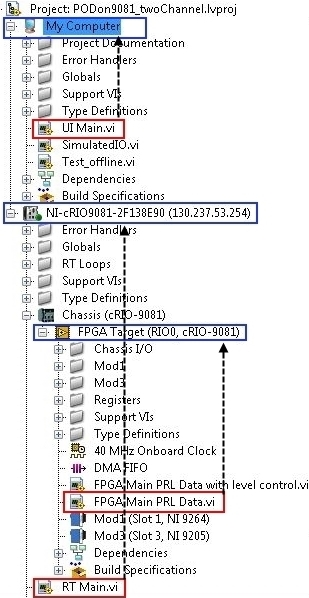
\includegraphics[width=3.1in,height=5in]{LabVIEWProj.JPG} 
\caption{LabVIEW Project explorer showing where different sections of code are run}
%\vspace{-0.6em}
\label{Two_area}
\end{figure}
\subsection{UI Main.vi} The first and primary VI was called UI Main and corresponds to Label 1 in Figure \ref{Final_arch}. A screenshot of the interface of this VI is shown in Figure \ref{Screenshot}. This serves are the main interface to the POD algorithm and allows for monitoring algorithm inputs, outputs and the performance of the cRIO. This VI is responsible for handling communication between the host computer (My Computer, in Figure \ref{Two_area}) and the cRIO (NI-cRIO9081 in Figure \ref{Two_area}). Data extracted from the PDC stream is read in this VI and is sent over the network to the cRIO. Errors generated by the POD algorithm are also received and stored here. Parameters required for the POD algorithm are entered and displayed here. Presently, the selection of the input signal for the POD algorithm is also performed here. This can be automated in future.
\subsection{RT Main.vi}
This VI runs on the real-time section of the cRIO at a loop rate of 5ms. It has no user interface as data is transmitted over the network and displayed on the remote computer. The primary function of this VI is to act as an intermediary between the POD algorithm running on the FPGA and the user interface on the remote computer. The input to the POD algorithm is received over the network and passed to the FPGA. As such, this VI is designed to be 'headless' and does not require the user interface to be active. In the present implementation, this cannot be achieved as the input to the POD algorithm is generated on the remote computer. Further development is needed to be able to unwrap the PMU data stream on the RT controller itself. Default values of the POD control parameters are stored and the algorithm itself can run without any action from the user. Network errors and latency are also handled here. Logging information and errors can be buffered temporarily before transmission over the network.
\subsection{FPGA Main.vi}
This section of code runs on the FPGA and primarily consists of the POD algorithm itself. Additionally, debug, data logging and error checking code is written to ensure that the algorithm responds only to user input. The code here is optimised and compiled for the limited resources available on the FPGA. This is also the only section of code that directly interacts with hardware. The output of the POD algorithm is directly written to the analogue output module in the cRIO. The loop rate here is 50$\mu s$. To account for the difference in loop rates between the FPGA and the RT section, a sample and hold algorithm is also implemented here.
%A set-up identical to that outlined in Figure \ref{Data_path} was constructed and used to verify the working of the real-time implementation of the Phasor-POD algorithm. The algorithm had previously been tested with the two area system within a \textsc{Simulink} environment (no HIL execution). It was verified to be able to keep the system in steady state stability and to restore the system to stability after the application of a minor disturbance. The benchmark for the real-time implementation of the algorithm is thus established. The single-line-diagram of the two-area test network used is shown in Figure \ref{Two_area} with PMU locations shown by the red buses. The signal generated from the real-time Phasor POD implementation is reinserted in the model at the control system of the SVC.
%\begin{figure}[htb]
%\centering
%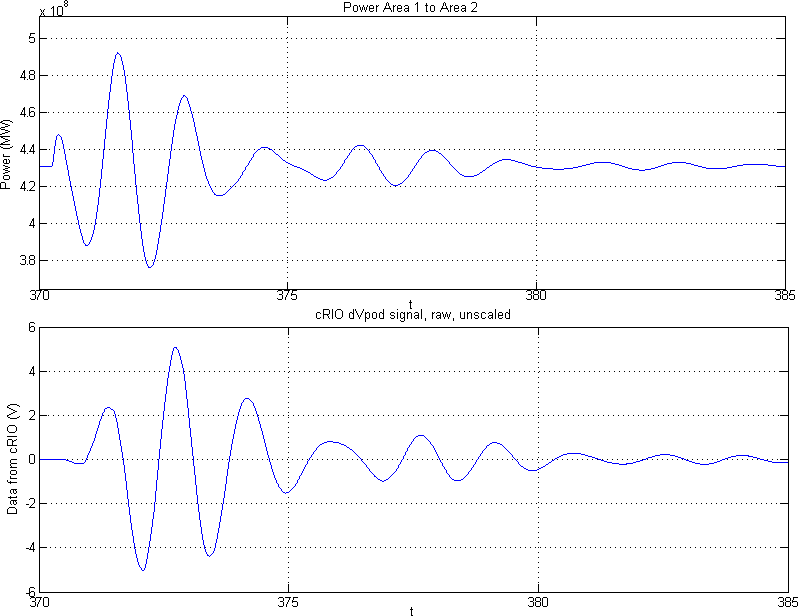
\includegraphics[width=3.5in]{Results.png} 
%\vspace{-0.6em}
%\caption{Performance of Hardware controller with small disturbance. Note that the decreasing magnitude of the damping signal indicates that the oscillation magnitude is decreasing in correspondence.}
%%\vspace{-0.5em}
%\label{Results}
%\end{figure}
%The hardware implementation of the POD algorithm was verified to be able to keep the system stable in steady state. It was also tested with small perturbations applied at one generator to excite the inter-area mode and was verified to work satisfactorily. Figure \ref{Results} shows the performance of the controller with two different inputs,active power and voltage angle difference. It is immediately evident that using the voltage angle difference provides better performance. Though this performance is not identical to that observed in simulations, it indicates that the real-time implementation of the algorithm was successful. 

%\vspace{-1em}
\section{Conclusion \& Results} \label{conclusion}
\subsubsection*{Note}Figure \ref{Data_path} shows an outline of the HIL test constructed to verify the working of the developed controller. The results are not examined in detail here due to constraints of space. The reader is, however, referred to \cite{Rebello} for a presentation of the results.

A hardware prototype of a real-time power oscillation damping control system was developed and tested. The developed prototype uses a real-time implementation of a wide-area control system. Issues and challenges faced in this implementation are documented and examined. The architecture development \& refinement process for this implementation is also examined in detail. The final software implementation resulting from this process was coded in LabVIEW and is presented. The success of the tests performed indicates that PMU-based wide area controllers can be exploited for multiple control applications in power system control and monitoring. % The damping signal generated by the hardware controller was captured on an oscilloscope and is presented in Figure \ref{ScopeCapture}.


% conference papers do not normally have an appendix


% use section* for acknowledgement
%\section*{Acknowledgment}
%The work of E. Rebello \& M.S. Almas was supported by the STRON$g^{2}$rid project, funded by Nordic Energy Research.\\
%L. Vanfretti is supported by the STRON$g^{2}$rid project, funded by Nordic Energy Research, and by the STandUP for Energy collaboration initiative and by Statnett SF, the Norwegian transmission system operator.
% trigger a \newpage just before the given reference
% number - used to balance the columns on the last page
% adjust value as needed - may need to be readjusted if
% the document is modified later
%\IEEEtriggeratref{8}
% The "triggered" command can be changed if desired:
%\IEEEtriggercmd{\enlargethispage{-5in}}
%\section*{Acknowledgment}
%\vspace{-1em}
%\begin{figure}[!htb]
%\centering
%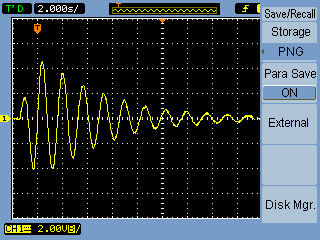
\includegraphics[width=3in]{Best_sample.png}
%\vspace{-0.6em}
%\caption{Controller Response with Voltage Angle Difference input captured using an Oscilloscope}
%\label{ScopeCapture}
%\end{figure}
% references section

% can use a bibliography generated by BibTeX as a .bbl file
% BibTeX documentation can be easily obtained at:
% http://www.ctan.org/tex-archive/biblio/bibtex/contrib/doc/
% The IEEEtran BibTeX style support page is at:
% http://www.michaelshell.org/tex/ieeetran/bibtex/
%\bibliographystyle{IEEEtran}
% argument is your BibTeX string definitions and bibliography database(s)
%\bibliography{IEEEabrv,../bib/paper}
%
% <OR> manually copy in the resultant .bbl file
% set second argument of \begin to the number of references
% (used to reserve space for the reference number labels box)
\begin{figure*}[b]
	\centering
	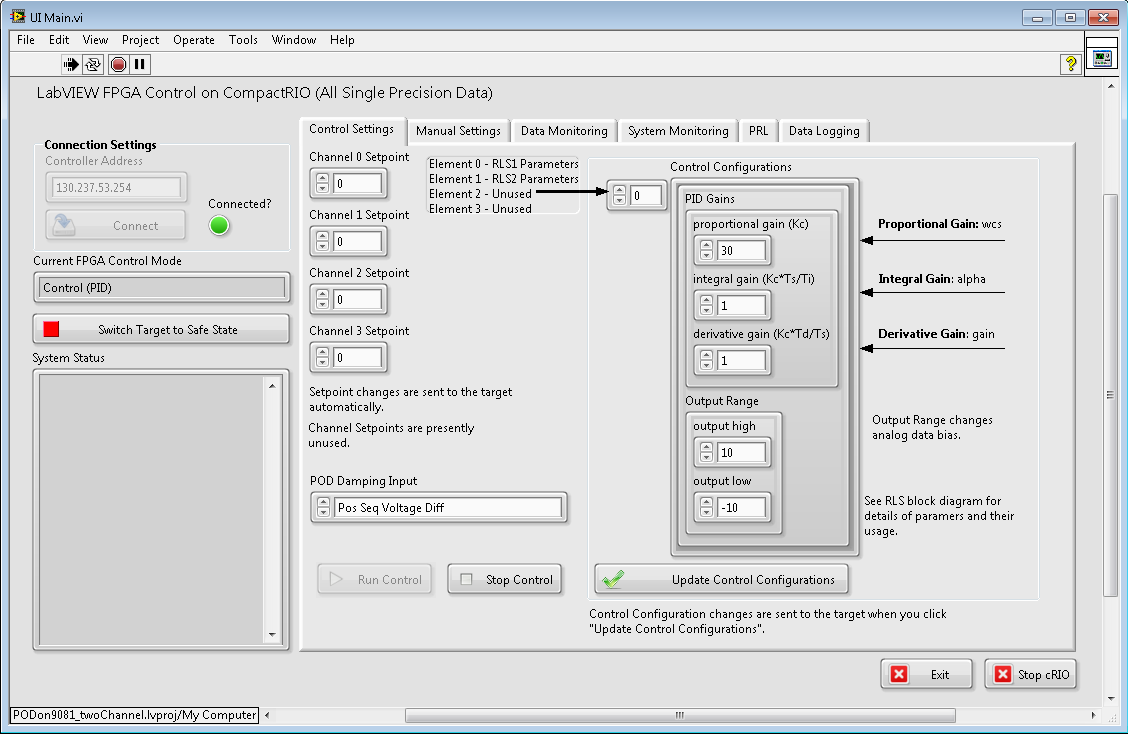
\includegraphics[width=6in]{Screenshot.png} 
	%	\vspace{-0.5em}
	\caption{User interface of \emph{UI Main.vi} showing control buttons, parameter setting, tabbed sections and damping input selection box.}
	\label{Screenshot}
\end{figure*}

\begin{thebibliography}{1}

\bibitem{NAERC} North American Electric Reliability Council \emph{Review of selected 1996 Electric System Disturbances in North America,} August 2002. Available Online: \url{http://www.nerc.com/pa/rrm/ea/System\%20Disturbance\%20Reports20DL/1996SystemDisturbance.pdf}

\bibitem{WAPODNorway} K. Uhlen, L.~Vanfretti, M.M. De Oliveira, A.B. Leirbukt,V. H. Aarstrand and J. O. Gjerde \emph{Wide-Area Power Oscillation Damper implementation and testing in the Norwegian transmission network} in Power and Energy Society General Meeting, 2012 IEEE pp. 1-7

\bibitem{localREMcomparison}  M. E.~Aboul-Ela, A. A.~Sallam, J. D.~McCalley and A. A.~Fouad, \emph{Damping Controller Design for Power System Oscillations Using Global Signals}, IEEE trans. on Power Systems, Vol. 11, No. 2, May 1996, pp. 767-773

\bibitem{Yuwa}  L.~Vanfretti, Y.~Chompoobutrgool, and J.H.~Chow, \emph{Chapter 10: Inter-Area Mode Analysis for Large Power Systems using Synchrophasor Data}, Book Chapter, in Coherency and Model Reduction of Large Power Systems, Joe H. Chow (Ed.), Springer, 2013.

\bibitem{WAPODChina} Li Peng and Wu Xiaochen and Lu Chao and Shi Jinghai and Hu Jiong and He Jingbo and Zhao Yong and Aidong Xu \emph{Implementation of CSG's Wide-Area Damping Control System: Overview and experience} in Power Systems Conference and Exposition, 2009. PSCE '09. IEEE/PES pp. 1-9

\bibitem{PhasorPOD} L.~\"{A}ngquist and C.~Gama  \emph{Damping Algorithm based on Phasor Estimation} in Power Engineering Society Winter Meeting, 2001. IEEE, Volume 3, pp. 1160 - 1165  

\bibitem{TaskForce} M.Crow, M. Gibbard, A. Messina, J. Pierre, J. Sanchez-Gasca, D. Trudnowski, D. Vowles \emph{Identification of Electromechanical Modes in Power Systems} IEEE Task Force Report, Special Publication TP462, June2012.

\bibitem{PhasorPODImplement} M.~Shoaib Almas and L.~Vanfretti, \emph{Implementation of Conventional PSS and Phasor Based POD for Power Stabilizing Controls for Real-Time Simulation}, IEEE IES IECON14, 29 Oct-1 Nov, 2014, Dallas, USA.

\bibitem{KundurTwoArea} 
M.~Klein, J. G.~Rogers and P.~Kundur \emph{A fundamental study of inter-area oscillations in Power Systems} IEEE Trans, PWRS, no. 6, pp. 914-921, 1991.

\bibitem{OPALemegasim} eMEGAsim PowerGrid Real-Time Digital Hardware in the Loop Simulator — Opal-RT, [Online]. Available: \url{http://www.opal-rt.com/}

\bibitem{cRIO9081} \emph{Operating Instructions and Specifications Compact RIO NI cRIO-9075/9076 \& NI cRIO-9081/9082}, National Instruments, Available Online at \url{http://www.ni.com/}

\bibitem{PMUMario} M. Paolone, A. Borghetti, C. A. Nucci, \emph{A Synchrophasor Estimation Algorithm for the Monitoring of Active Distribution Networks in Steady State and Transient Conditions}, Proc. of the 17th Power Systems Computation Conference (PSCC 2011), Stockholm, Sweden, Aug. 22-26, 2011 

\bibitem{SIMULINKOnline} Kamwa \ I. (Hydro-Quebec) "Performance of Three PSS for Interarea Oscillations" Available Online at : \url{http://www.mathworks.se/help/physmod/sps/examples_v2/performance-of-three-pss-for-interarea-oscillations.html}

%\bibitem{eMEGASIM} \emph{eMEGASIM Power Grid Real-Time Digital HArdware in the Loop Simulator} Available Online at : \url{http://www.opal-rt.com/}

%\bibitem{Dmello} F. P.~Dmello, and C.~Concordia \emph{Concepts of Synchronous Machine Stability as Affected by Excitation Control} IEEE Transactions on Power Apparatus and Systems, vol. PAS 88, no. 4, 1969. 

\bibitem{SmarTSLab} M.S. Almas, M. Baudette, L. Vanfretti, S. Lovlund and J.O. Gjerde "\emph{Synchrophasor network, laboratory and software applications developed in the STRON$g^{2}$rid project}," PES General Meeting, Conference Exposition, July 2014 IEEE pp 1 - 5

\bibitem{WaterfallCoding} James Taylor \emph{Managing Information Technology Projects : Applying Project Management Strategies to Software, Hardware, and Integration Initiatives}, AMACOM Books, September 2003 pp 237-239

\bibitem{Rebello} E. Rebello, L. Vanfretti and M.S Almas \emph{PMU-based Real-Time Damping Control System Software and Hardware Architecture Synthesis and Evaluation} IEEE PES GM, Denver, Colorado, July 2015,

%\bibitem{Chaudhuri} N.S.~Chaudhuri, R.~Majumder and B~ Chaudhuri \emph{Interaction between conventional and adaptive phasor power oscillation damping controllers} in Power and Energy Society General Meeting, 2010 IEEE Minneapolis, MN, 2012 pp. 1-7

%\bibitem{sVARdamp} E.V~Larsen and E.H~Chow, General Electric Company, NY, \emph{SVC control design concepts for system dynamic performance}, in Application of Static Var Systems for System Dynamic Performance 1987, IEEE, pp. 36-53

%\bibitem{cRIO9076} \emph{Operating Instructions and Specifications Compact RIO NI cRIO-9075/9076}, National Instruments, Available Online at \url{http://www.ni.com/pdf/manuals/375650b.pdf}

%\bibitem{LabviewTemplate} \emph{FPGA Control on Compact RIO Sample Project Documentation}, National Instruments, Available Online at \url{http://www.ni.com/white-paper/14137/en/}

\bibitem{SDK} L. Vanfretti, V.H. Aarstrand, M. Shoaib Almas, V. S. Peri\'c and J.O Gjerde \emph{A Software Development Toolkit for Real-Time Synchrophasor Applications},  IEEE PES Grenoble PowerTech, 2013

%\bibitem{MATLABexample} I~Kamwa \emph{Performance of Three PSS for Interarea Oscillations} SimPowerSystems Examples, \textsc{Matlab} R2011a

%\bibitem{PSSDocumentation} \emph{Generic Power System Stabilizer} Documentation distributed with \textsc{Matlab} R2014a Available online at \url{http://www.mathworks.se/help/physmod/sps/powersys/ref/genericpowersystemstabilizer.html}

%\begin{figure}[]
%\centering
%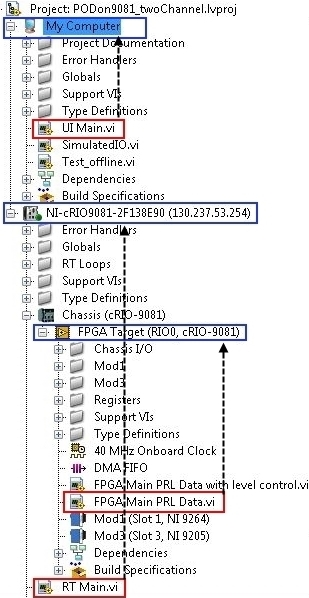
\includegraphics[width=3in]{LabVIEWProj.JPG}
%\caption{LabView Project Explorer showing different sections of code and the devices on which they run. \textbf{This image is too tall to fit within the text. I wanted to include this as an appendix but the Latex file says that conference papers generally don't have appendices.
%}}
%\label{LabProject}
%\end{figure}

\end{thebibliography}

\end{document}


